\documentclass[UTF8]{ctexrep}
\usepackage{fontspec}
\usepackage{graphicx}
\usepackage{listings}
\usepackage{gbt7714}

\setmainfont{Times New Roman}
\graphicspath{{figures/}}

\title{ViT-MNIST Report}
\date{}

\begin{document}
\maketitle

% content
\chapter{程序}
\section{原理介绍}
Vision Transformer(ViT)由Dosovitskiy等人\cite{dosovitskiy2021an}提出,
Transformer是自然语言处理(Natural Language Processing, NLP)中常见的模型,
而在计算机视觉(Computer Vision, CV)领域,注意力机制的应用范围仍然较小,
通常是替换卷积神经网络(Convolutional Neural Network, CNN)中的一部分组件,同时保持其整体结构不变。
作者等人发现对CNN的依赖是毫无必要的,在图像分类任务上单纯使用Transformer能够带来更好的效果。

\begin{figure}[htbp]
    \centering
    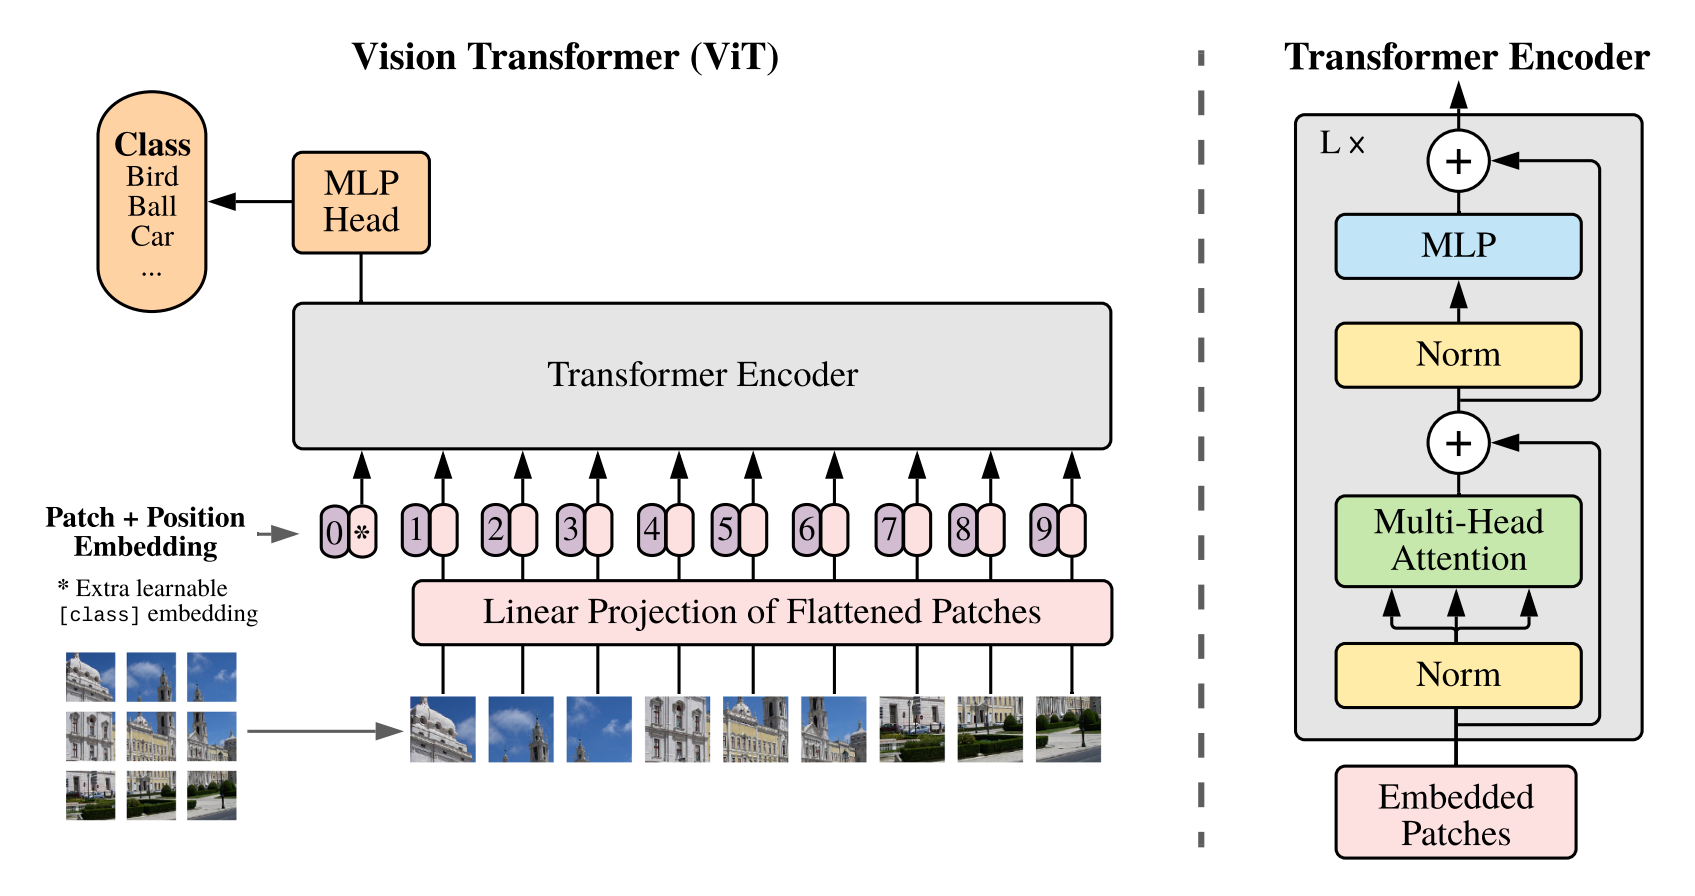
\includegraphics[width=0.9\linewidth]{model-overview.png}
    \caption{模型结构}
    \label{fig:model-overview}
\end{figure}

模型结构如~\ref{fig:model-overview}所示,首先目标图片被划分为几个大小相同的patch,
线性组合后输入到一个标准的Transformer Encoder中,在输入到一个多层感知器(Multi-Layer Perceptron, MLP)中得到分类的结果。

本实验中,ViT的实现依赖了开源项目vit-pytorch\cite{vit-torch}。

\section{实现细节}
如图~\ref{fig:init}所示是ViT模型中\_\_init\_\_方法的代码,定义了模型的结构,与~\ref{fig:model-overview}所示结构一致。

\begin{figure}[htbp]
    \centering
    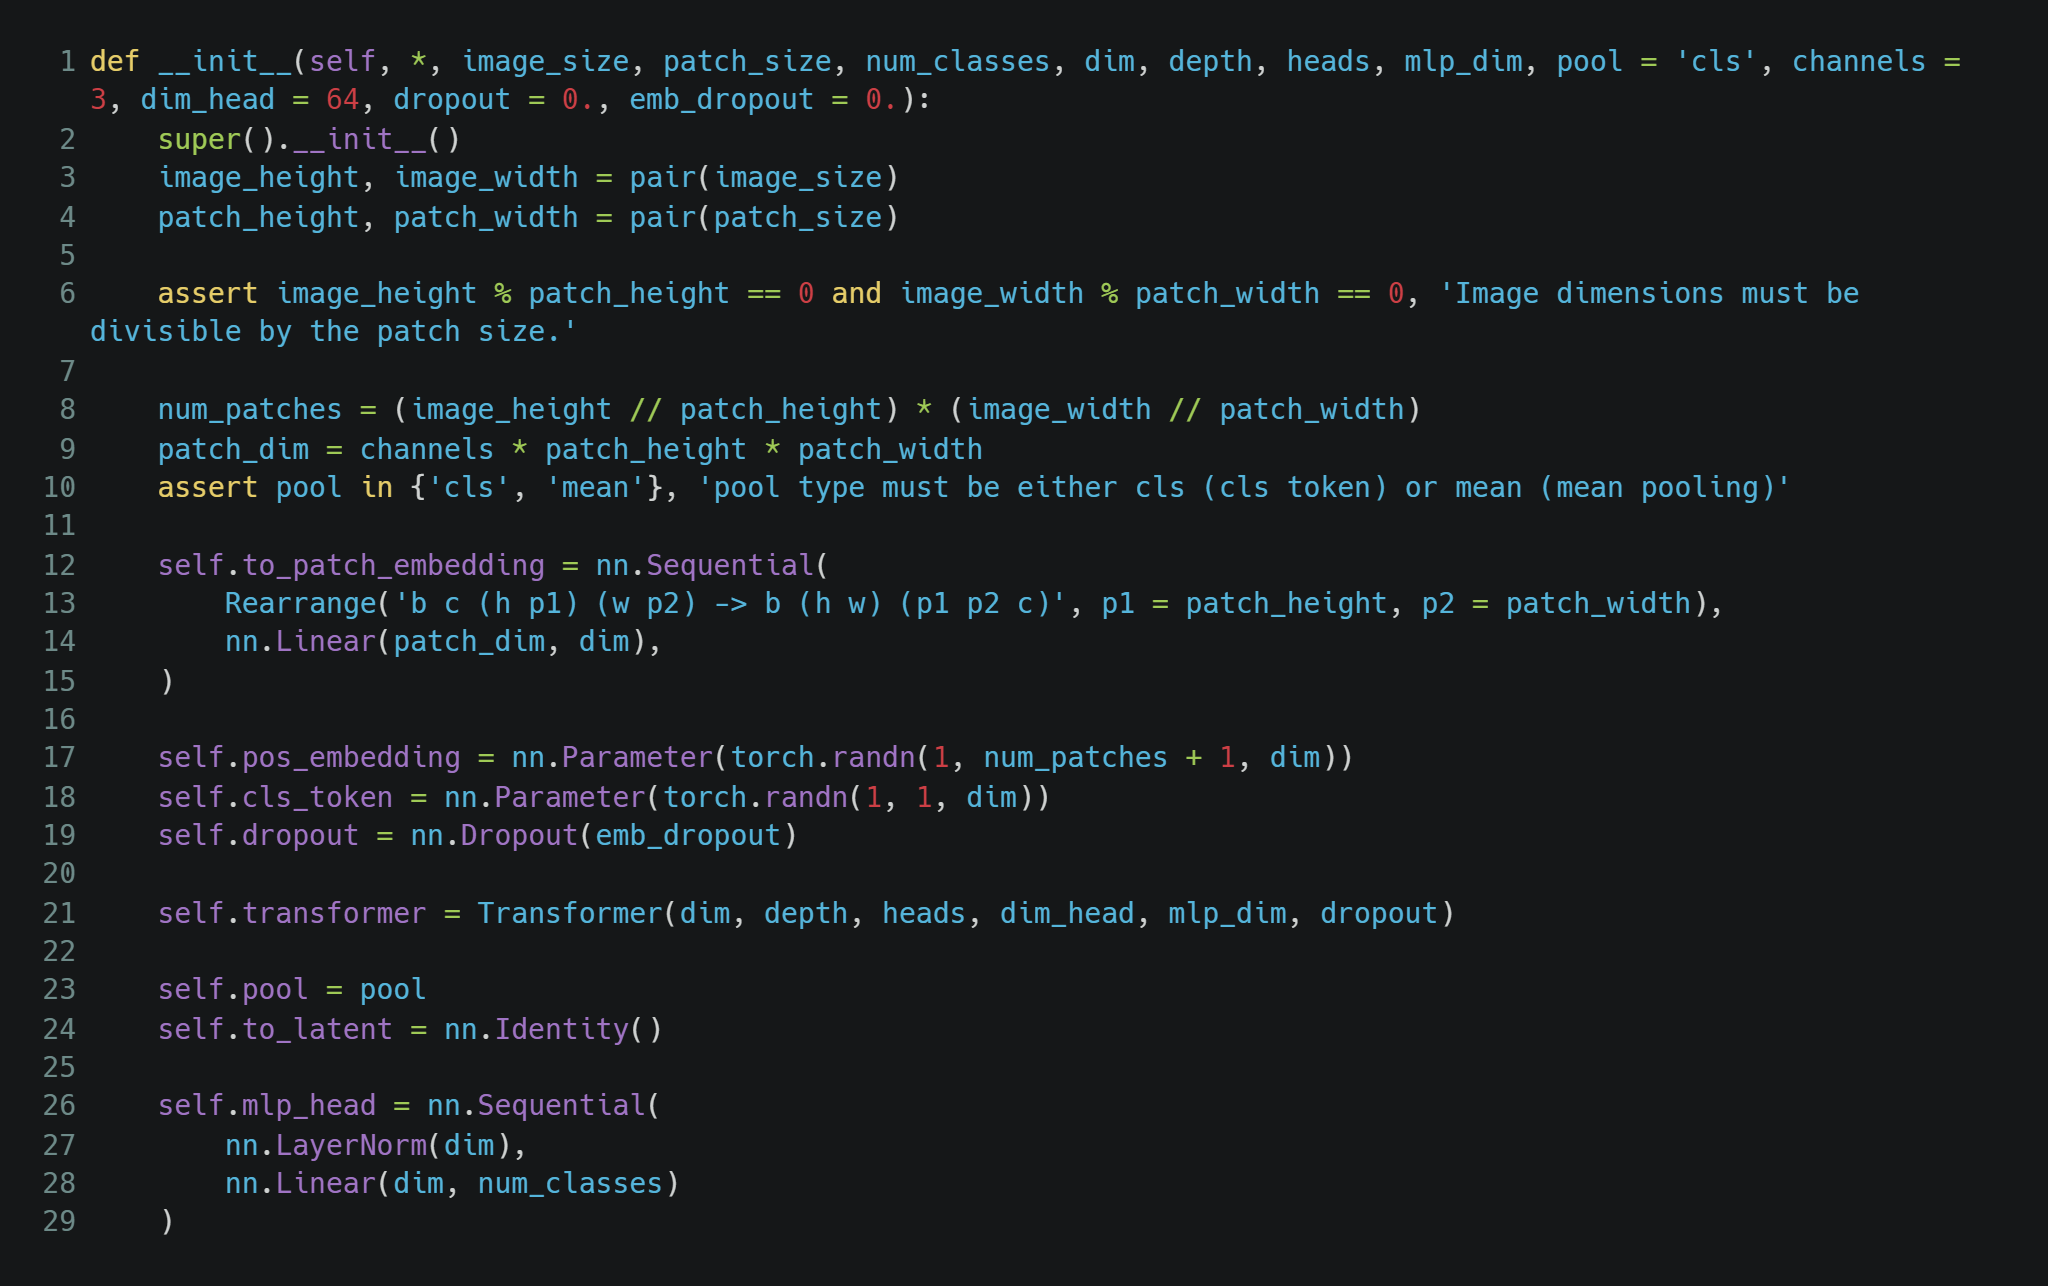
\includegraphics[width=0.9\linewidth]{init.png}
    \caption{\_\_init\_\_代码}
    \label{fig:init}
\end{figure}

如图~\ref{fig:forward}所示是ViT模型中forward方法的代码,描述了模型正向传播的过程。

\begin{figure}[htbp]
    \centering
    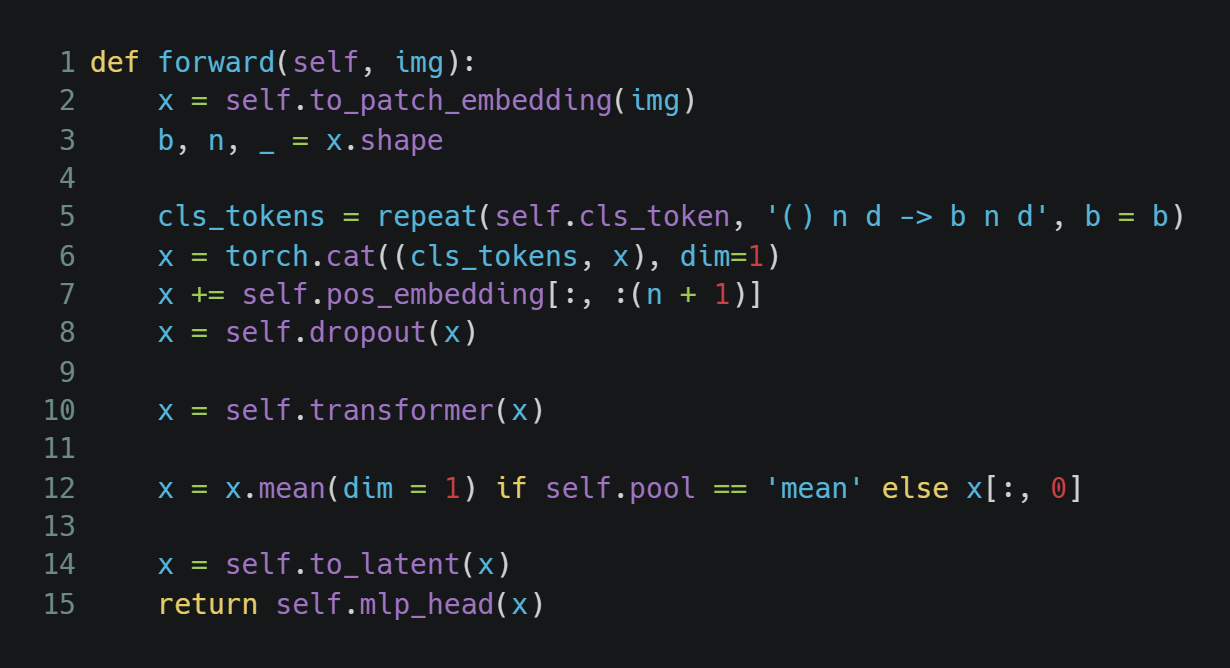
\includegraphics[width=0.9\linewidth]{forward.png}
    \caption{forward代码}
    \label{fig:forward}
\end{figure}

如图~\ref{fig:train-epoch}所示是训练一个epoch的代码。

\begin{figure}[htbp]
    \centering
    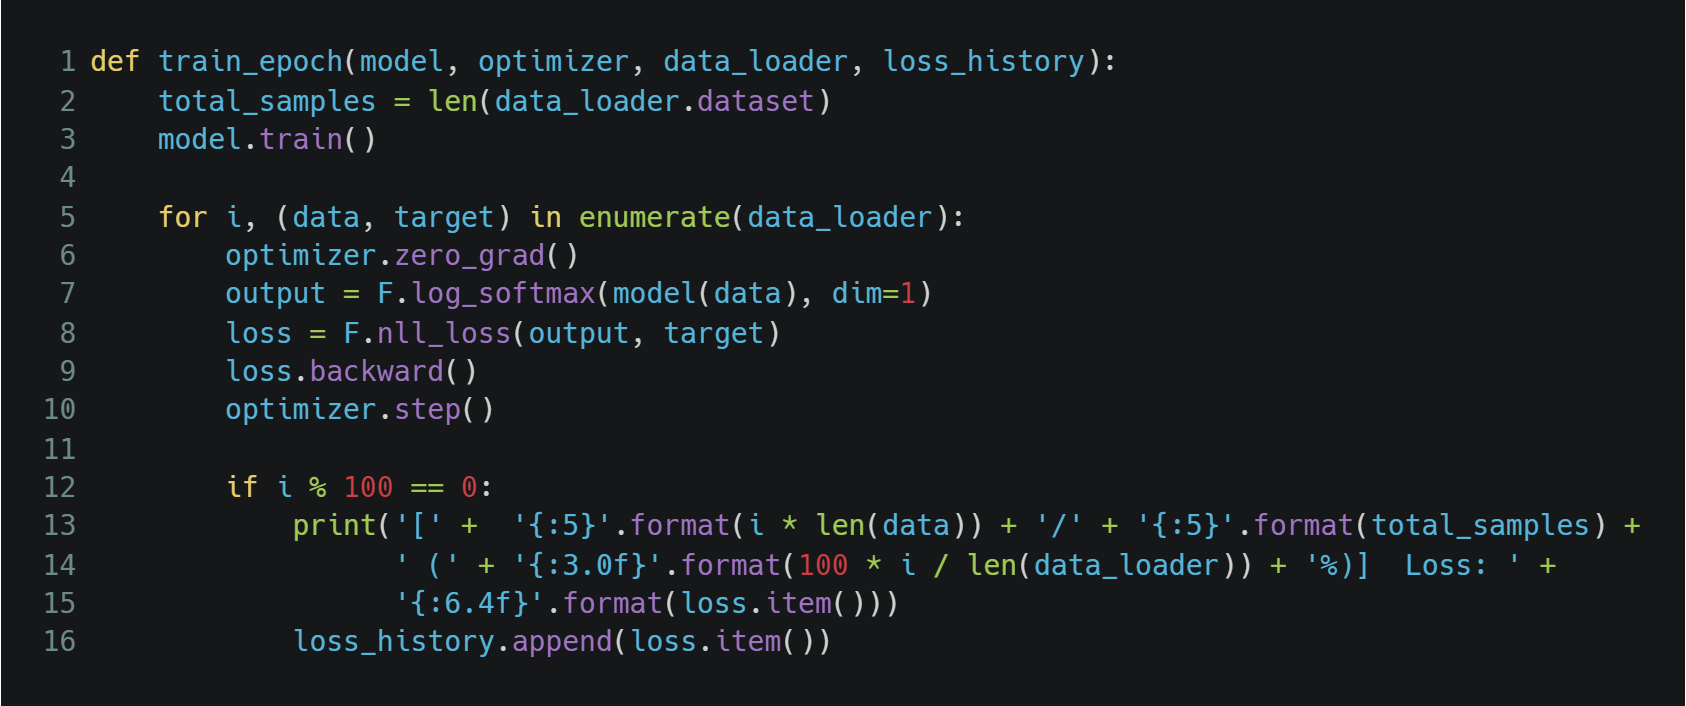
\includegraphics[width=0.9\linewidth]{train-epoch.png}
    \caption{train\_epoch代码}
    \label{fig:train-epoch}
\end{figure}

\chapter{结果}
经过25个epoch的训练后效果如图~\ref{fig:result}所示。
\begin{figure}
    \centering
    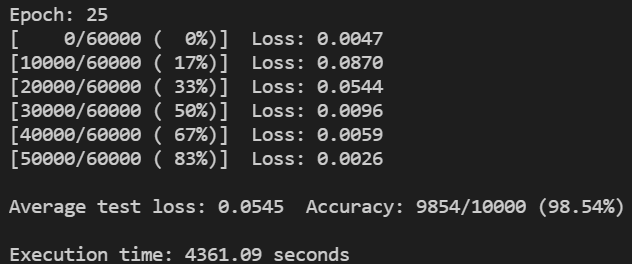
\includegraphics[width=0.9\linewidth]{result.png}
    \caption{result}
    \label{fig:result}
\end{figure}

\graphicspath{{../}}
train loss如图~\ref{fig:train-loss}所示。
\begin{figure}
    \centering
    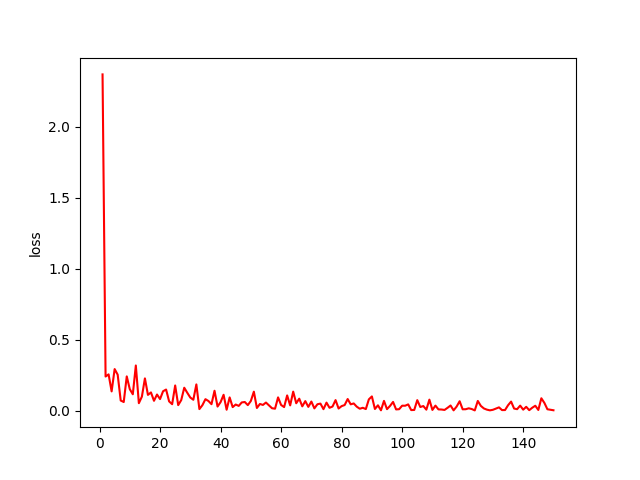
\includegraphics[width=0.9\linewidth]{train-loss.png}
    \caption{train loss}
    \label{fig:train-loss}
\end{figure}

test loss如图~\ref{fig:test-loss}所示。
\begin{figure}
    \centering
    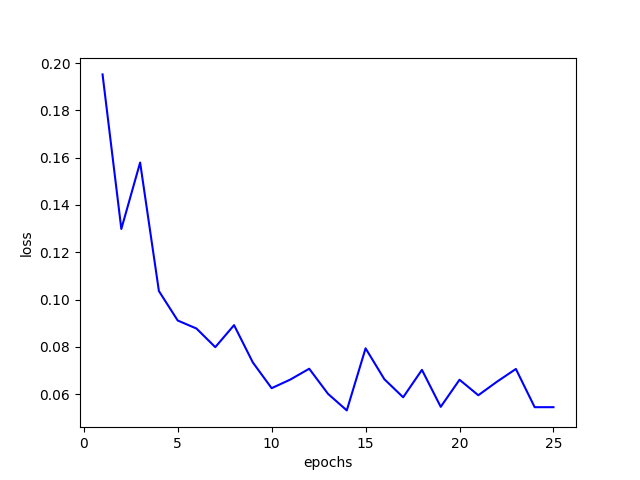
\includegraphics[width=0.9\linewidth]{test-loss.png}
    \caption{test loss}
    \label{fig:test-loss}
\end{figure}

\bibliographystyle{gbt7714-numerical}
\bibliography{reference}
\end{document}